%!TeX root=../wowtop.tex

\ArtChapter[The Heat-Ray]{5head}

\lettrine[lines=4,findent=2pt]{A}{fter} the glimpse I had had of the Martians emerging from the cylinder in which they had come to the earth from their planet, a kind of fascination paralysed my actions. I remained standing knee-deep in the heather, staring at the mound that hid them. I was a battleground of fear and curiosity.

I did not dare to go back towards the pit, but I felt a passionate longing to peer into it. I began walking, therefore, in a big curve, seeking some point of vantage and continually looking at the sand-heaps that hid these new-comers to our earth. Once a leash of thin black whips, like the arms of an octopus, flashed across the sunset and was immediately withdrawn, and afterwards a thin rod rose up, joint by joint, bearing at its apex a circular disk that spun with a wobbling motion. What could be going on there?

Most of the spectators had gathered in one or two groups—one a little crowd towards Woking, the other a knot of people in the direction of Chobham. Evidently they shared my mental conflict. There were few near me. One man I approached—he was, I perceived, a neighbour of mine, though I did not know his name—and accosted. But it was scarcely a time for articulate conversation.

»What ugly \textit{brutes}!« he said. »Good God! What ugly brutes!« He repeated this over and over again.

»Did you see a man in the pit?« I said; but he made no answer to that. We became silent, and stood watching for a time side by side, deriving, I fancy, a certain comfort in one another's company. Then I shifted my position to a little knoll that gave me the advantage of a yard or more of elevation and when I looked for him presently he was walking towards Woking.

% \begin{figure}[tbh!]
	% \centering
	% 
\includegraphics[width=\linewidth]{5heatray}
	% \caption{This invisible, inevitable sword of heat}
% \end{figure}

\begin{bwbigpic}
	[1.2] 
	{5heatray} 
	{This invisible, inevitable sword of heat} 
\end{bwbigpic}

The sunset faded to twilight before anything further happened. The crowd far away on the left, towards Woking, seemed to grow, and I heard now a faint murmur from it. The little knot of people towards Chobham dispersed. There was scarcely an intimation of movement from the pit.

It was this, as much as anything, that gave people courage, and I suppose the new arrivals from Woking also helped to restore confidence. At any rate, as the dusk came on a slow, intermittent movement upon the sand-pits began, a movement that seemed to gather force as the stillness of the evening about the cylinder remained unbroken. Vertical black figures in twos and threes would advance, stop, watch, and advance again, spreading out as they did so in a thin irregular crescent that promised to enclose the pit in its attenuated horns. I, too, on my side began to move towards the pit.

Then I saw some cabmen and others had walked boldly into the sand-pits, and heard the clatter of hoofs and the gride of wheels. I saw a lad trundling off the barrow of apples. And then, within thirty yards of the pit, advancing from the direction of Horsell, I noted a little black knot of men, the foremost of whom was waving a white flag.

This was the Deputation. There had been a hasty consultation, and since the Martians were evidently, in spite of their repulsive forms, intelligent creatures, it had been resolved to show them, by approaching them with signals, that we too were intelligent.

Flutter, flutter, went the flag, first to the right, then to the left. It was too far for me to recognise anyone there, but afterwards I learned that Ogilvy, Stent, and Henderson were with others in this attempt at communication. This little group had in its advance dragged inward, so to speak, the circumference of the now almost complete circle of people, and a number of dim black figures followed it at discreet distances.

Suddenly there was a flash of light, and a quantity of luminous greenish smoke came out of the pit in three distinct puffs, which drove up, one after the other, straight into the still air.

This smoke (or flame, perhaps, would be the better word for it) was so bright that the deep blue sky overhead and the hazy stretches of brown common towards Chertsey, set with black pine trees, seemed to darken abruptly as these puffs arose, and to remain the darker after their dispersal. At the same time a faint hissing sound became audible.

\begin{wrapfigure}{O}{0.5\textwidth}
\centering

\includegraphics[width=0.5\textwidth]{5flag}
%\captionlistentry{Waving a white flag}
\end{wrapfigure}

Beyond the pit stood the little wedge of people with the white flag at its apex, arrested by these phenomena, a little knot of small vertical black shapes upon the black ground. As the green smoke arose, their faces flashed out pallid green, and faded again as it vanished. Then slowly the hissing passed into a humming, into a long, loud, droning noise. Slowly a humped shape rose out of the pit, and the ghost of a beam of light seemed to flicker out from it.

Forthwith flashes of actual flame, a bright glare leaping from one to another, sprang from the scattered group of men. It was as if some invisible jet impinged upon them and flashed into white flame. It was as if each man were suddenly and momentarily turned to fire.

% \begin{sidewaysfigure}
	% 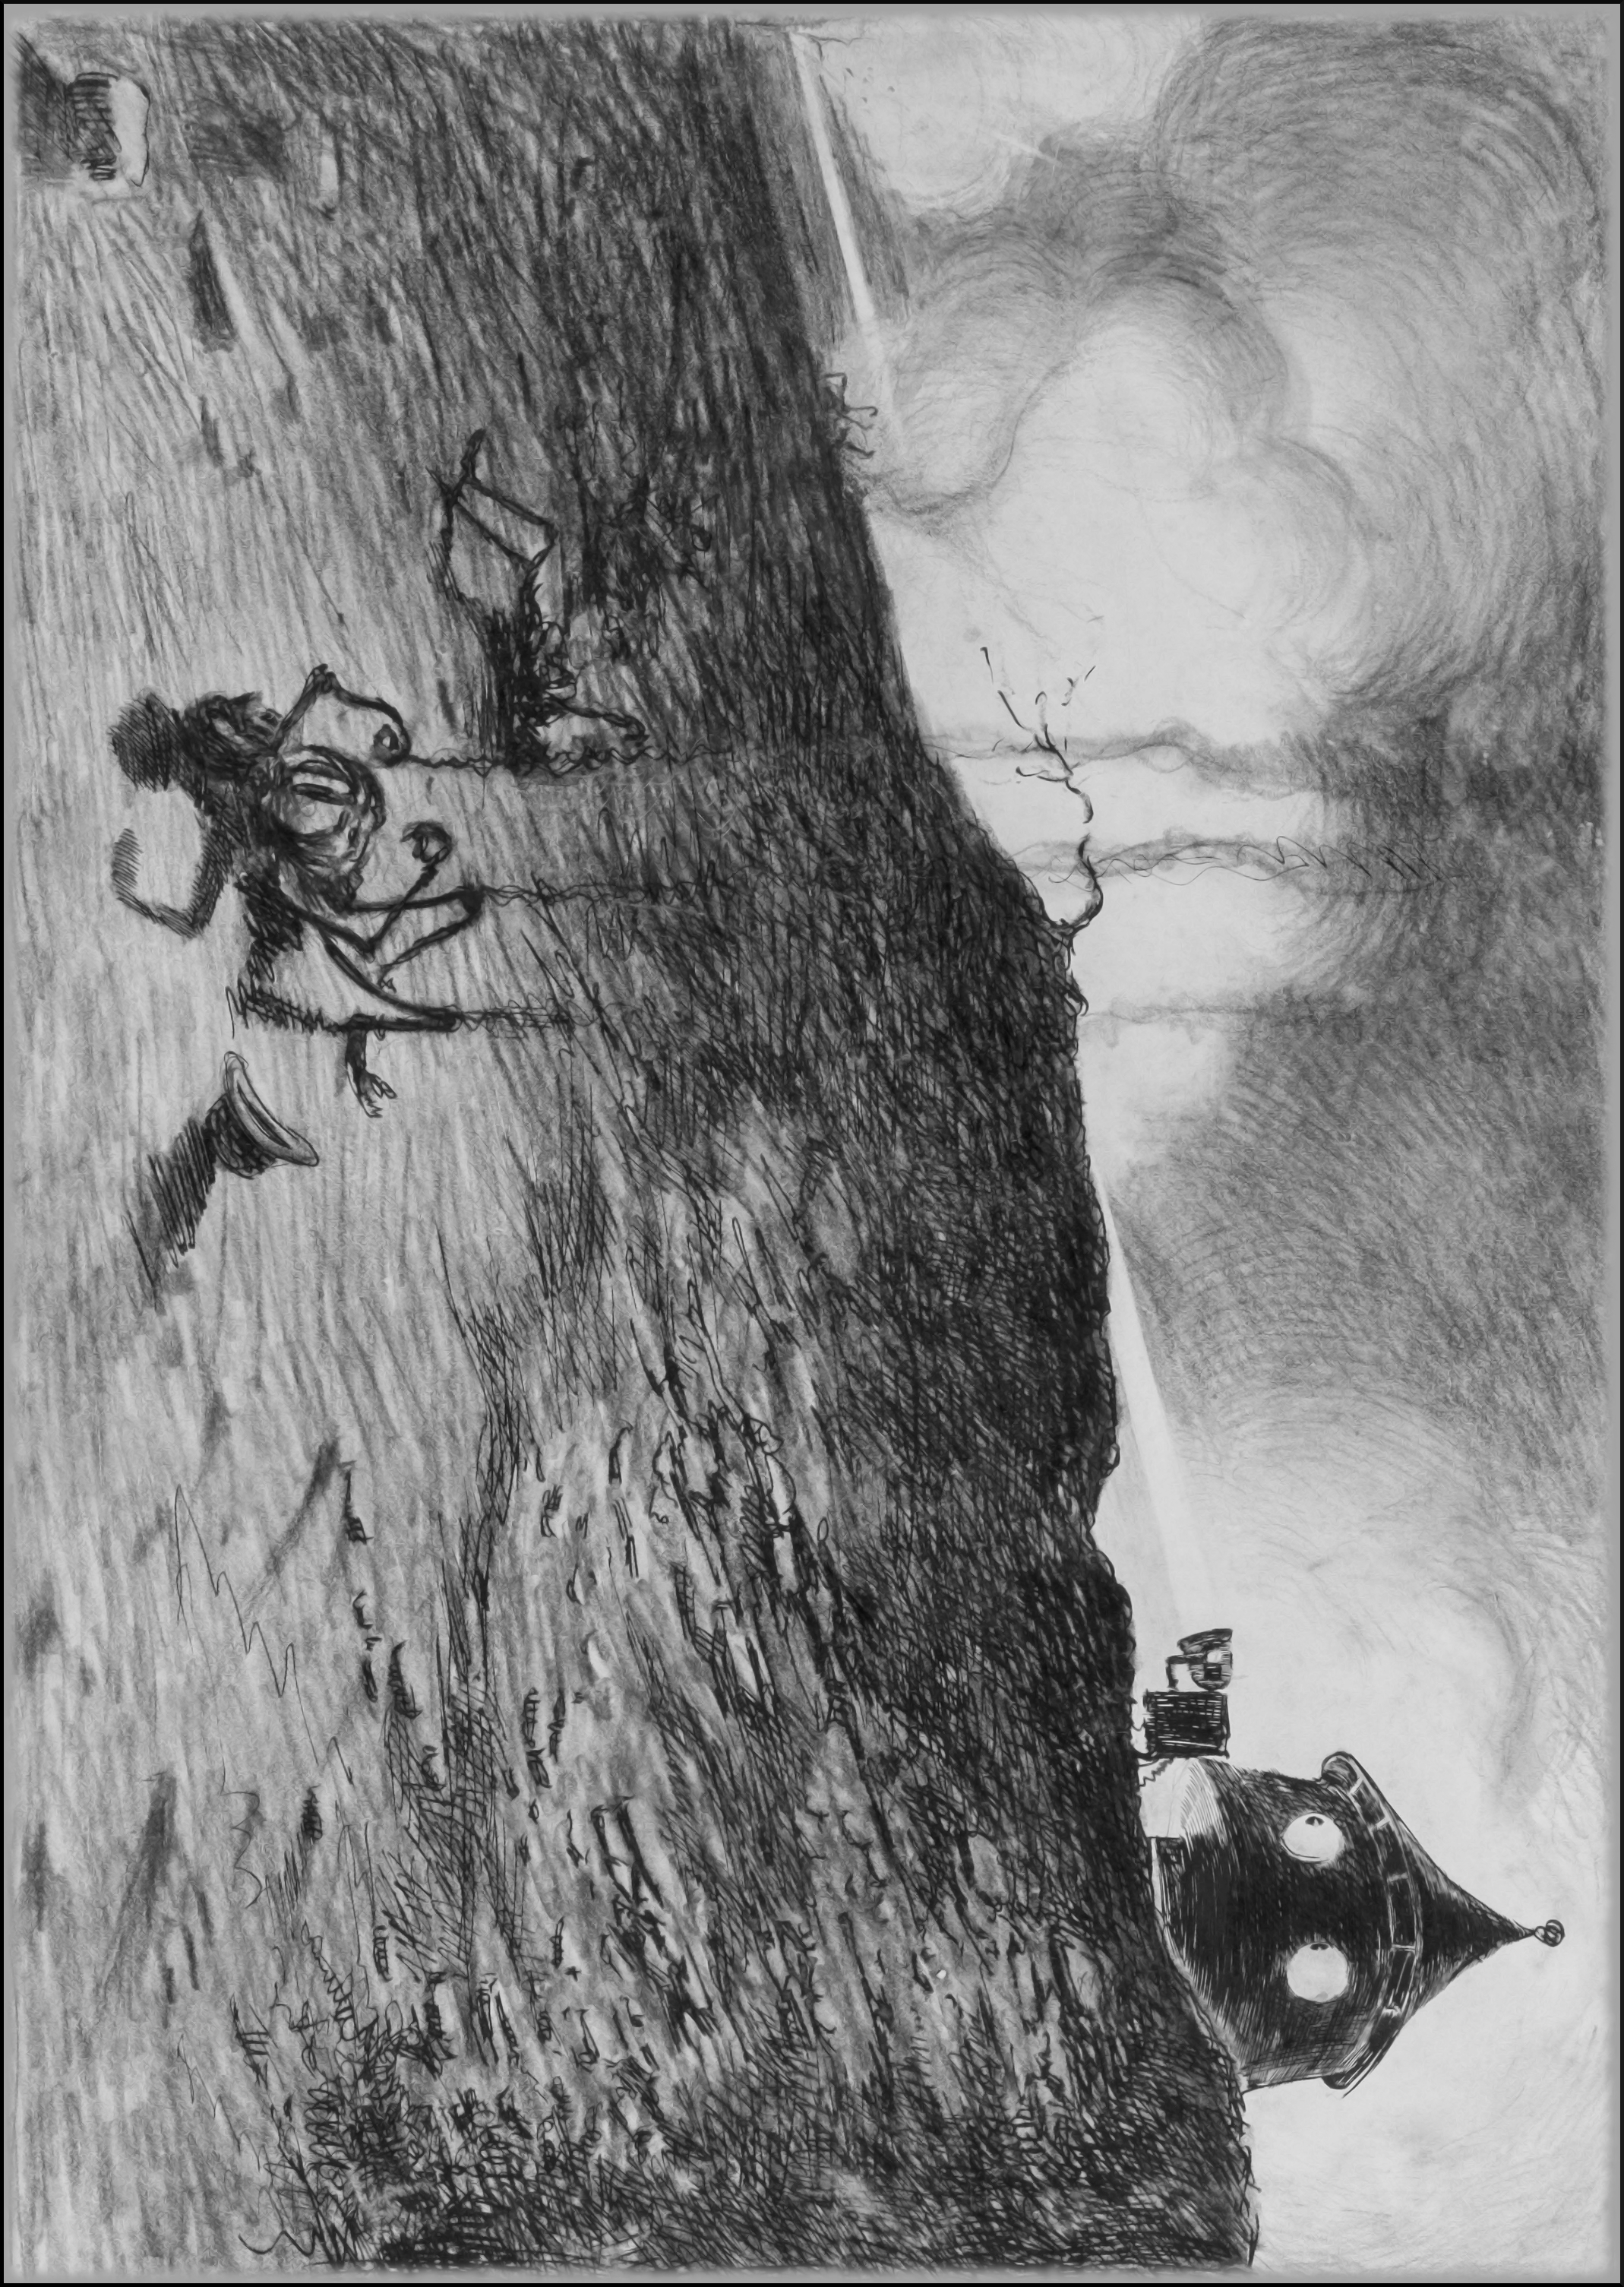
\includegraphics[width=\columnwidth]{5invisiblejet}%
% \caption[Flashed into white flame]{As if some invisible jet impinged upon them and flashed into white flame}
% \end{sidewaysfigure}



Then, by the light of their own destruction, I saw them staggering and falling, and their supporters turning to run.

I stood staring, not as yet realising that this was death leaping from man to man in that little distant crowd. All I felt was that it was something very strange. An almost noiseless and blinding flash of light, and a man fell headlong and lay still; and as the unseen shaft of heat passed over them, pine trees burst into fire, and every dry furze bush became with one dull thud a mass of flames. And far away towards Knaphill I saw the flashes of trees and hedges and wooden buildings suddenly set alight.

It was sweeping round swiftly and steadily, this flaming death, this invisible, inevitable sword of heat. I perceived it coming towards me by the flashing bushes it touched, and was too astounded and stupefied to stir. I heard the crackle of fire in the sand-pits and the sudden squeal of a horse that was as suddenly stilled. Then it was as if an invisible yet intensely heated finger were drawn through the heather between me and the Martians, and all along a curving line beyond the sand-pits the dark ground smoked and crackled. Something fell with a crash far away to the left where the road from Woking station opens out on the common. Forth-with the hissing and humming ceased, and the black, dome-like object sank slowly out of sight into the pit.



All this had happened with such swiftness that I had stood motionless, dumbfounded and dazzled by the flashes of light. Had that death swept through a full circle, it must inevitably have slain me in my surprise. But it passed and spared me, and left the night about me suddenly dark and unfamiliar.

The undulating common seemed now dark almost to blackness, except where its roadways lay grey and pale under the deep blue sky of the early night. It was dark, and suddenly void of men. Overhead the stars were mustering, and in the west the sky was still a pale, bright, almost greenish blue. The tops of the pine trees and the roofs of Horsell came out sharp and black against the western afterglow. The Martians and their appliances were altogether invisible, save for that thin mast upon which their restless mirror wobbled. Patches of bush and isolated trees here and there smoked and glowed still, and the houses towards Woking station were sending up spires of flame into the stillness of the evening air.

Nothing was changed save for that and a terrible astonishment. The little group of black specks with the flag of white had been swept out of existence, and the stillness of the evening, so it seemed to me, had scarcely been broken.

It came to me that I was upon this dark common, helpless, unprotected, and alone. Suddenly, like a thing falling upon me from without, came—fear.


\begin{pictures} %As if some invisible jet impinged upon them (letter)
	\begin{letter}
		\clearpage
		\begin{tikzpicture}[remember picture, overlay]
			\node (img) at ($(current page.center)+(0.5cm,0cm)$) {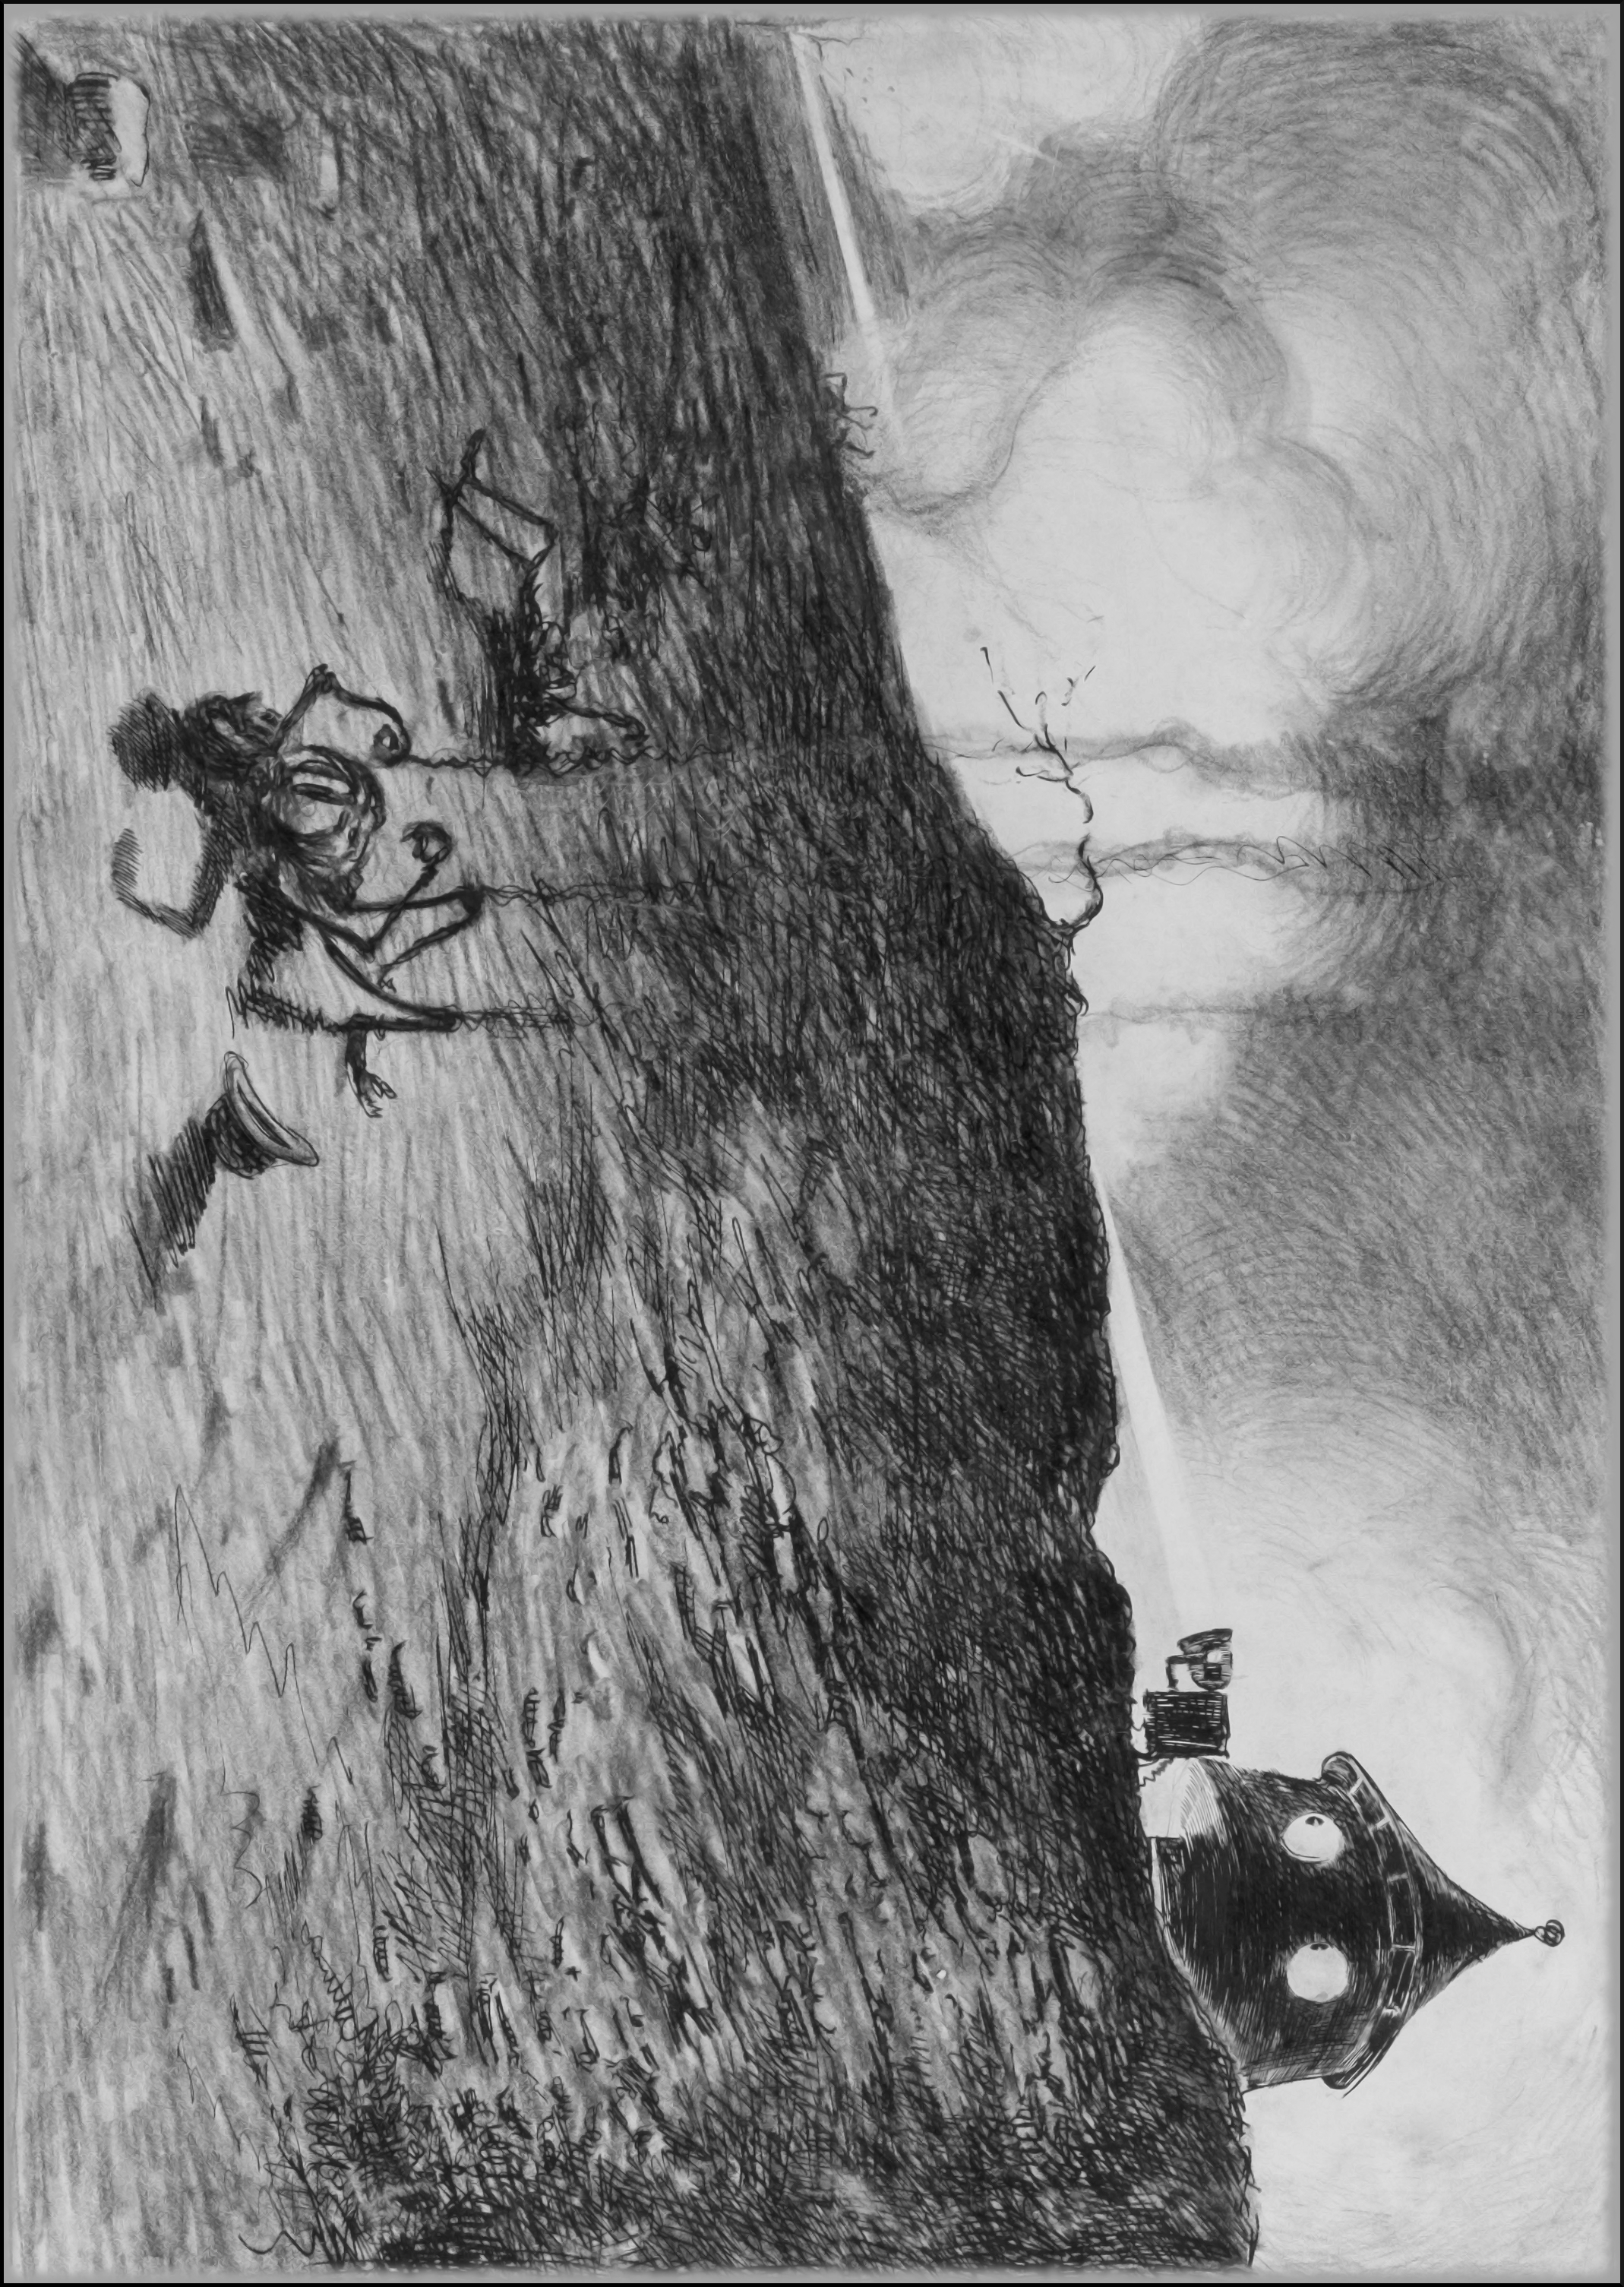
\includegraphics[width=1.15\columnwidth]{5invisiblejet}};
			\node[rotate=-90, text width=\textwidth, align=center] (caption) at ($(current page.west)+(1cm,0cm)$) {\textsc{As if some invisible jet impinged upon them}};

		\end{tikzpicture}
		\thispagestyle{empty}
		\addxcontentsline{lof}{figure}{As if some invisible jet impinged upon them}
		\clearpage
	\end{letter}
\end{pictures}



With an effort I turned and began a stumbling run through the heather.


\begin{pictures} %As if some invisible jet impinged upon them (a4)
	\begin{a4}
		\clearpage
		\begin{tikzpicture}[remember picture, overlay]
			\node (img) at ($(current page.center)+(0.5cm,0cm)$) {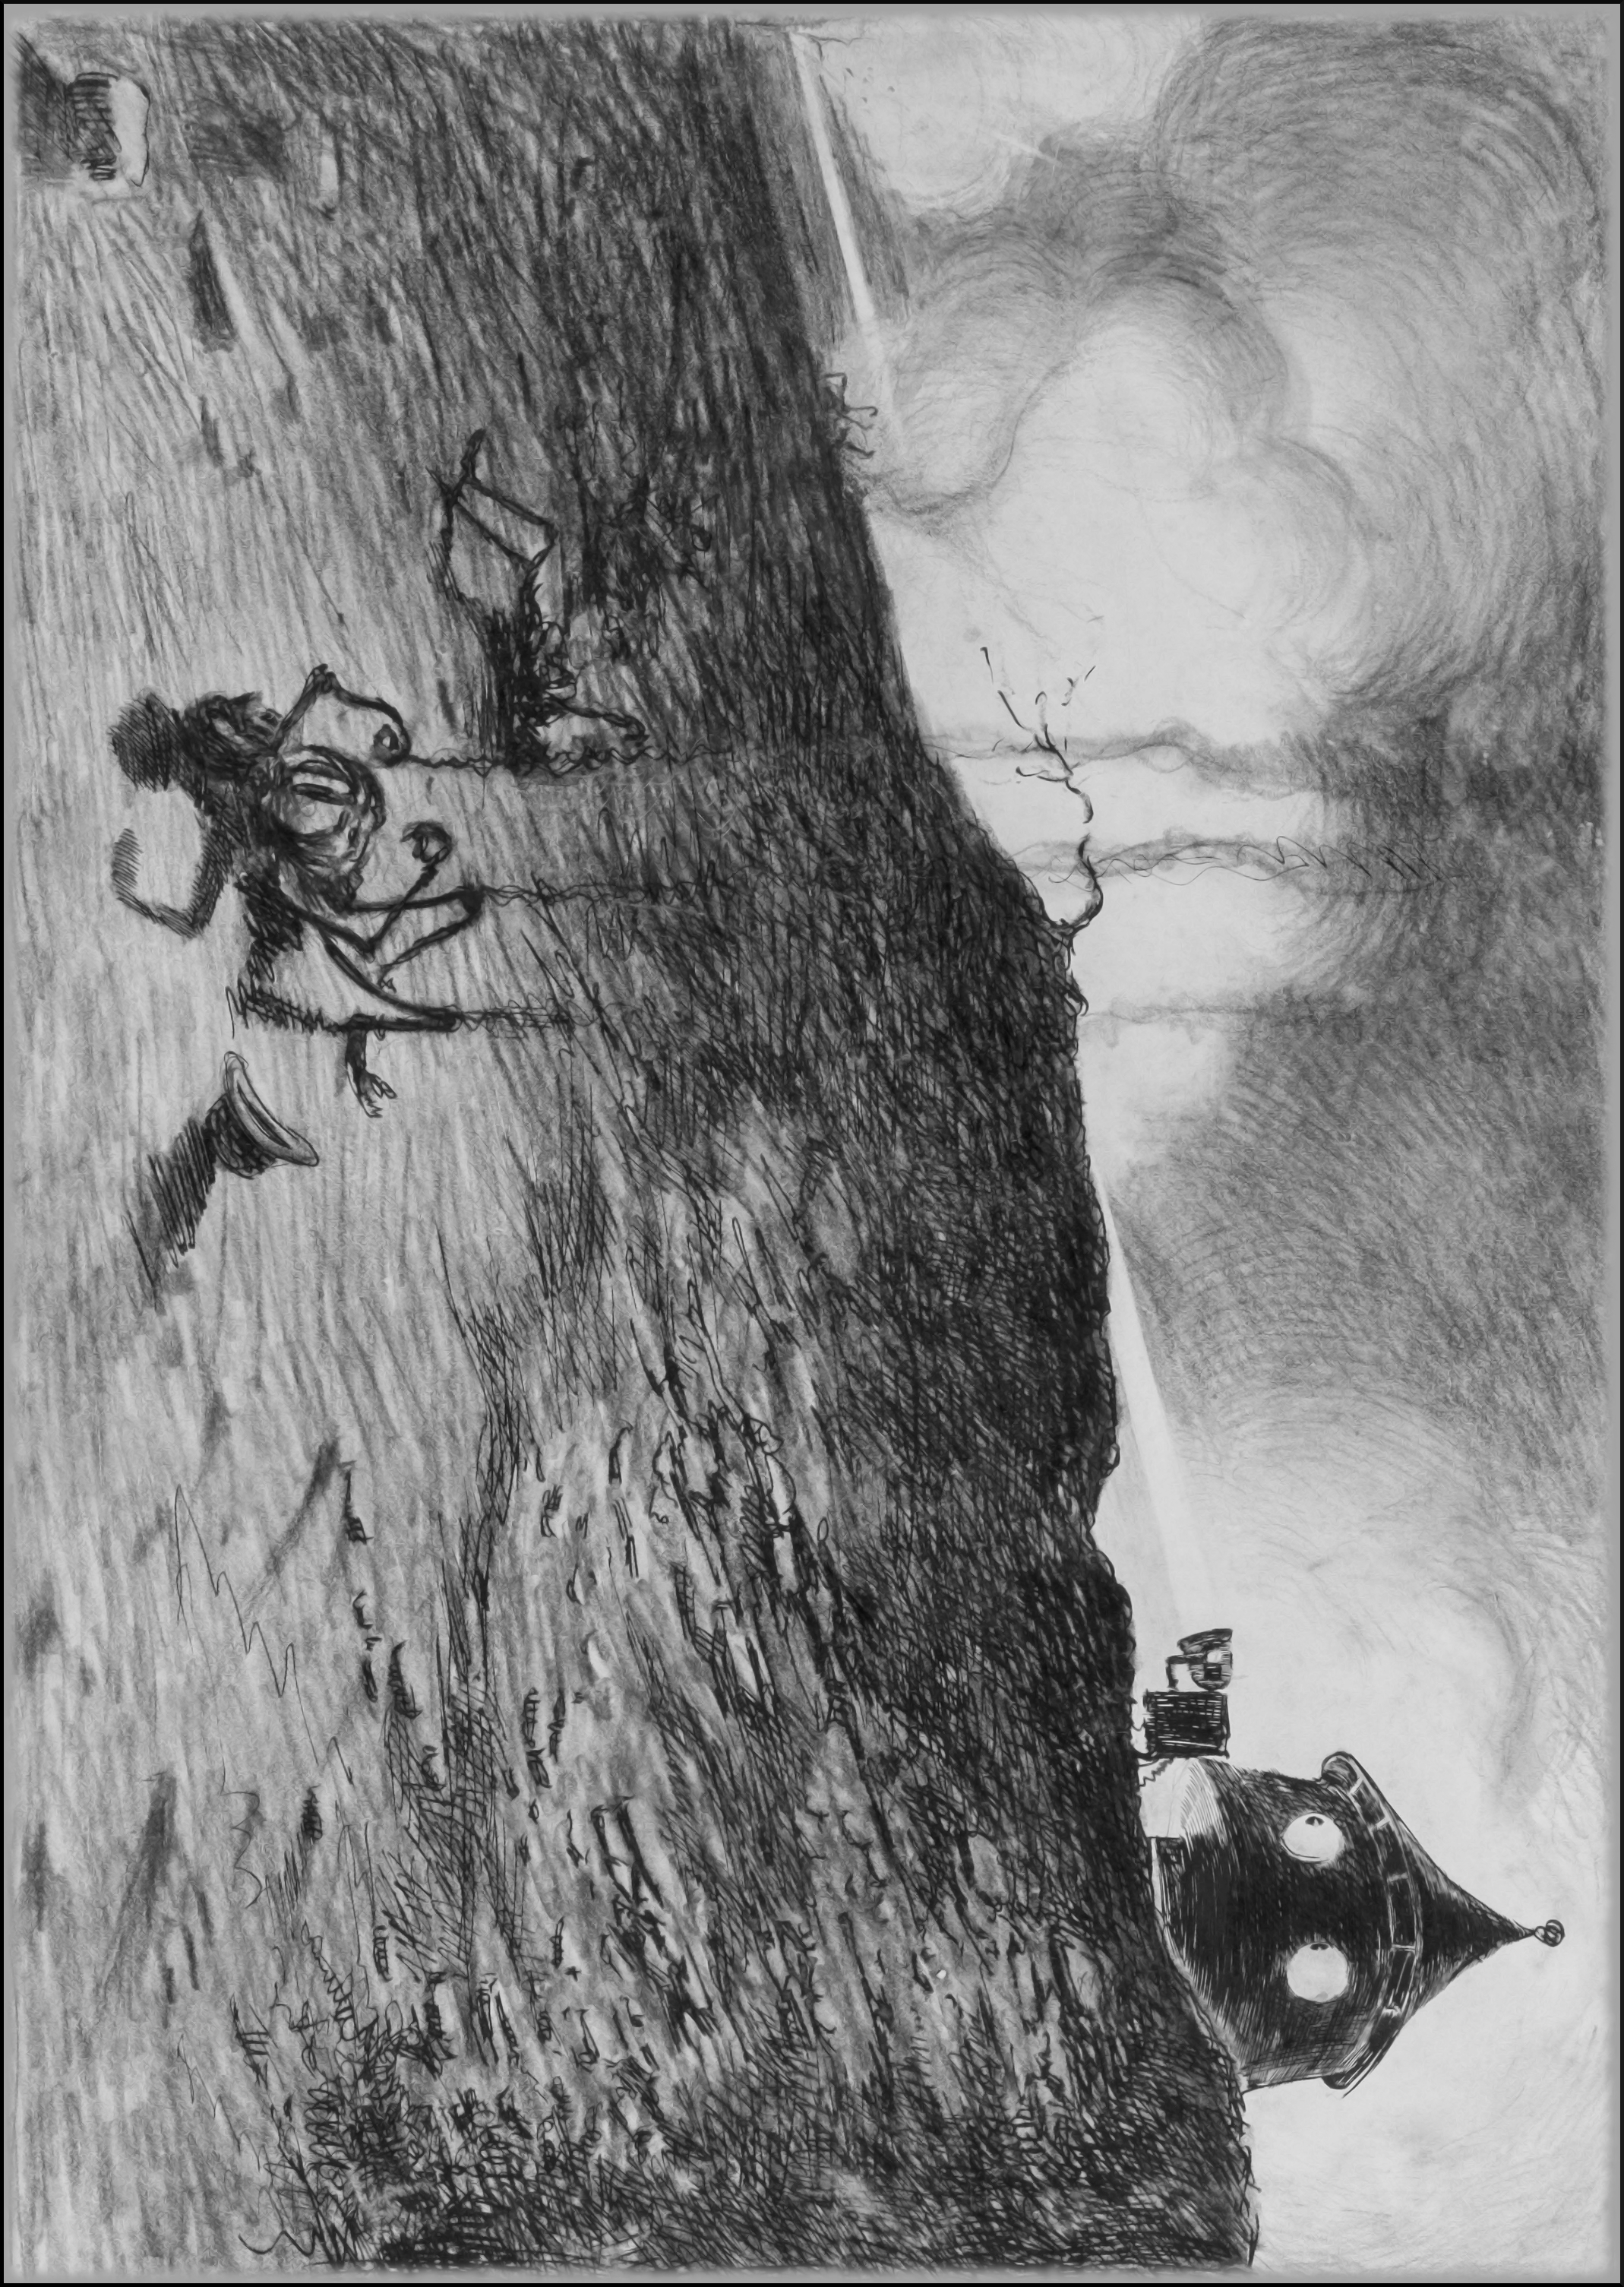
\includegraphics[width=1.15\columnwidth]{5invisiblejet}};
			\node[rotate=-90, text width=\textwidth, align=center] (caption) at ($(current page.west)+(1cm,0cm)$) {\textsc{As if some invisible jet impinged upon them}};

		\end{tikzpicture}
		\thispagestyle{empty}
		\addxcontentsline{lof}{figure}{As if some invisible jet impinged upon them}
		\clearpage
	\end{a4}
\end{pictures}

The fear I felt was no rational fear, but a panic terror not only of the Martians, but of the dusk and stillness all about me. Such an extraordinary effect in unmanning me it had that I ran weeping silently as a child might do. Once I had turned, I did not dare to look back.

I remember I felt an extraordinary persuasion that I was being played with, that presently, when I was upon the very verge of safety, this mysterious death—as swift as the passage of light—would leap after me from the pit about the cylinder, and strike me down.

\begin{figure}[b!]
\centering
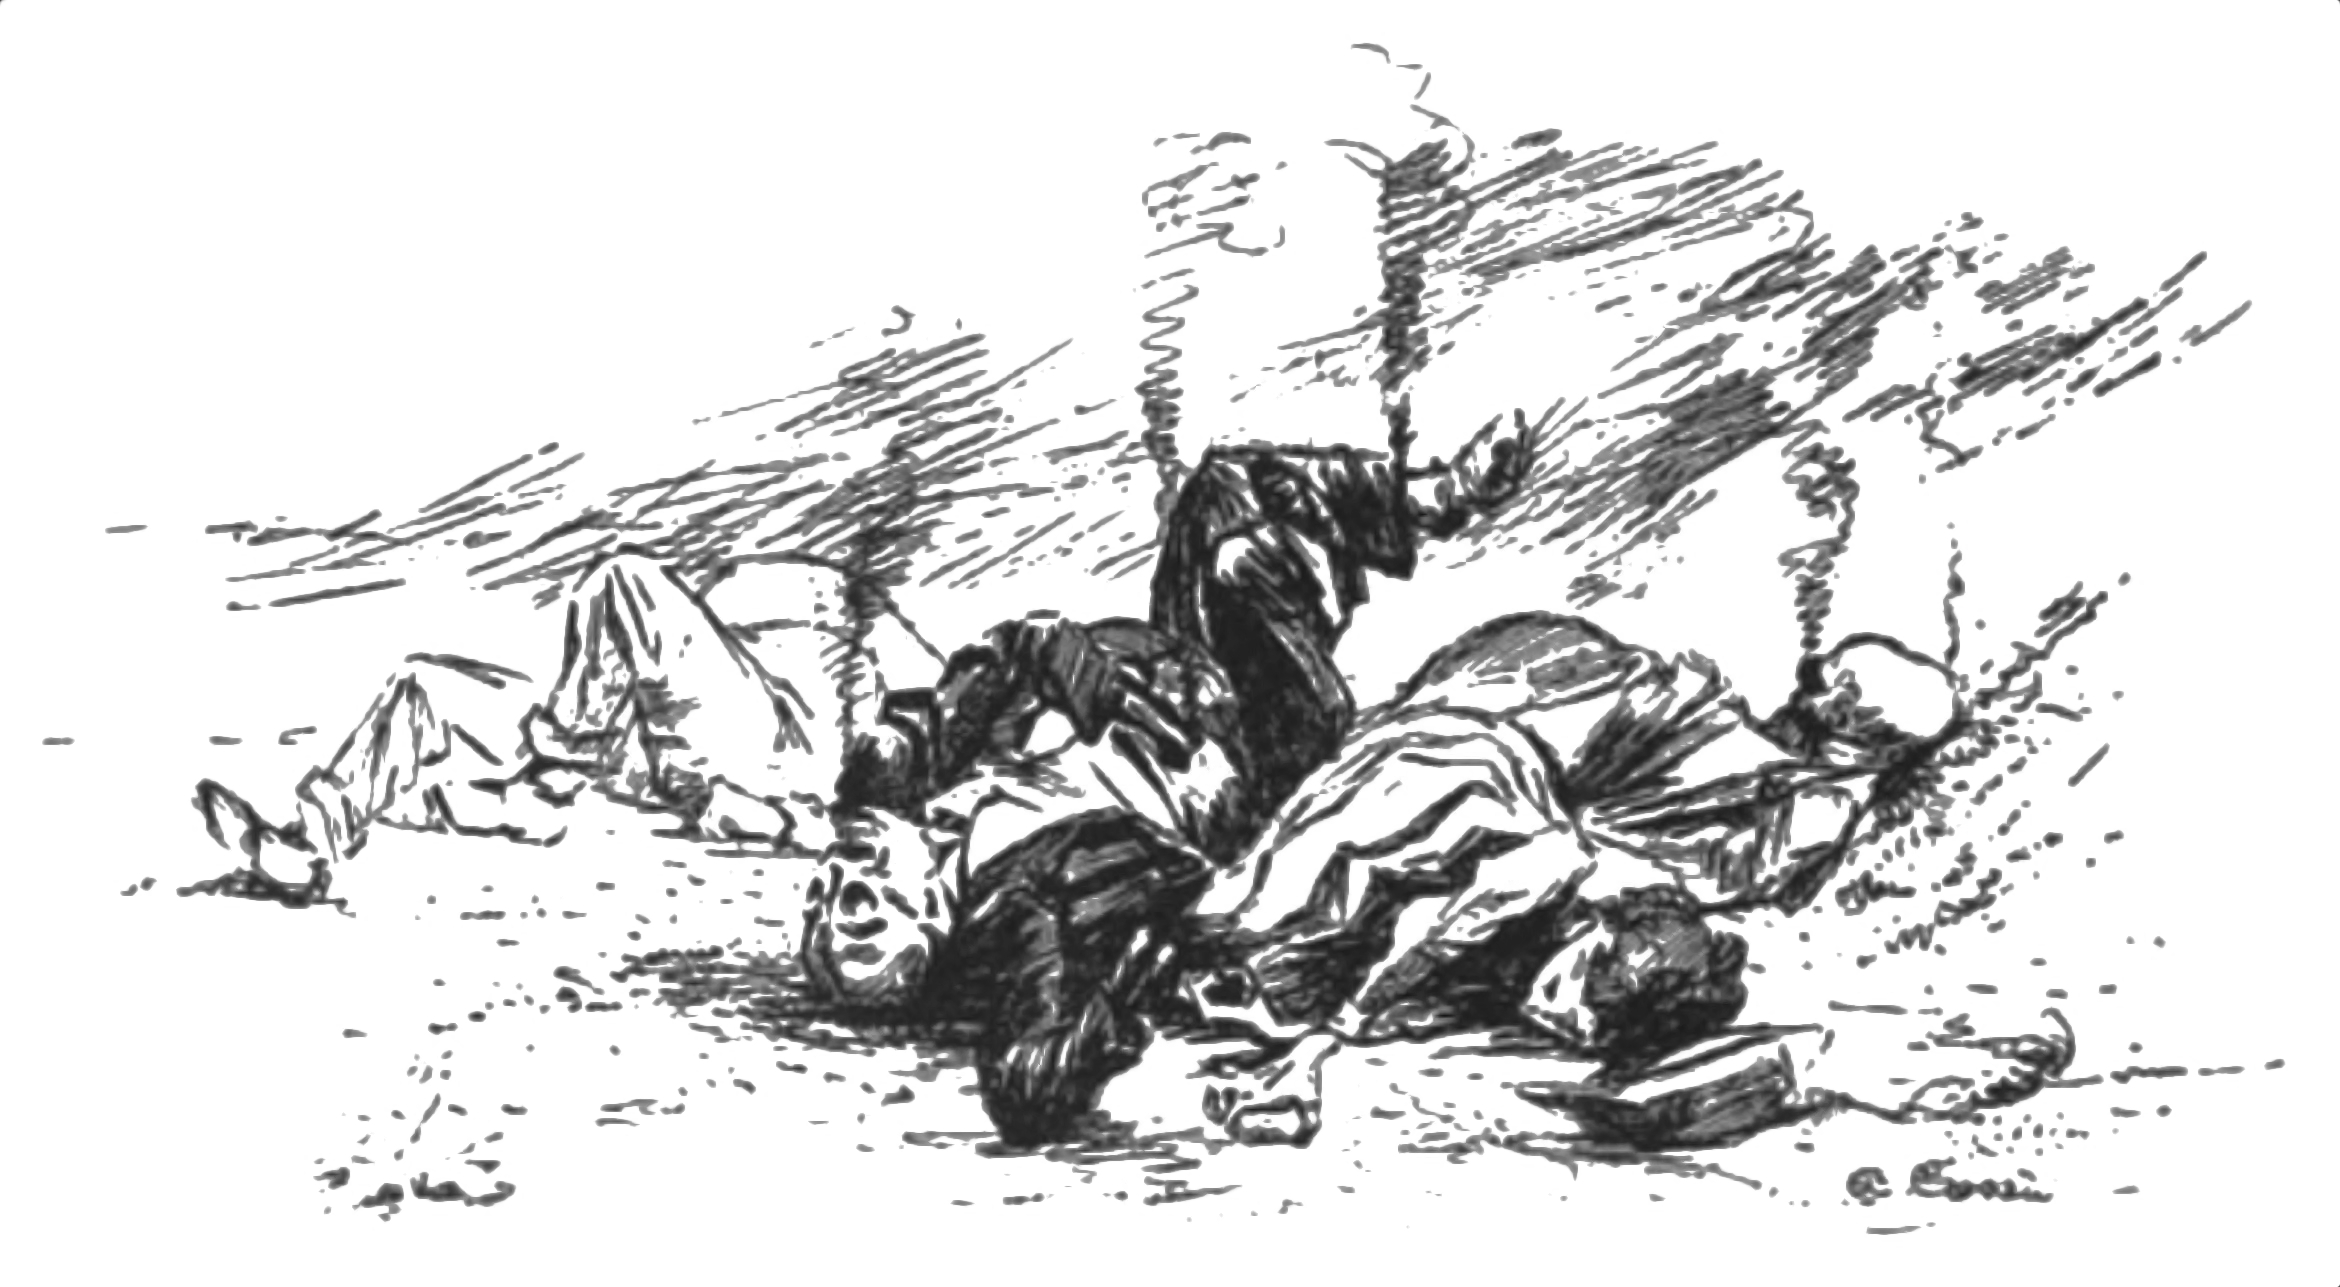
\includegraphics[width=.8\textwidth]{5tailpiece}
%\captionlistentry{Tailpiece to Chapter \thechapter}
\end{figure}